% CHAPTER 2 — STORYBOARDS
\chapter{Storyboards}
\label{cap:storyboards}

\section{Authentication and Personal Area}

\subsection{Login}
The login screen allows the user to authenticate by inserting their credentials (email and password).
\begin{figure}[H]
    \centering
    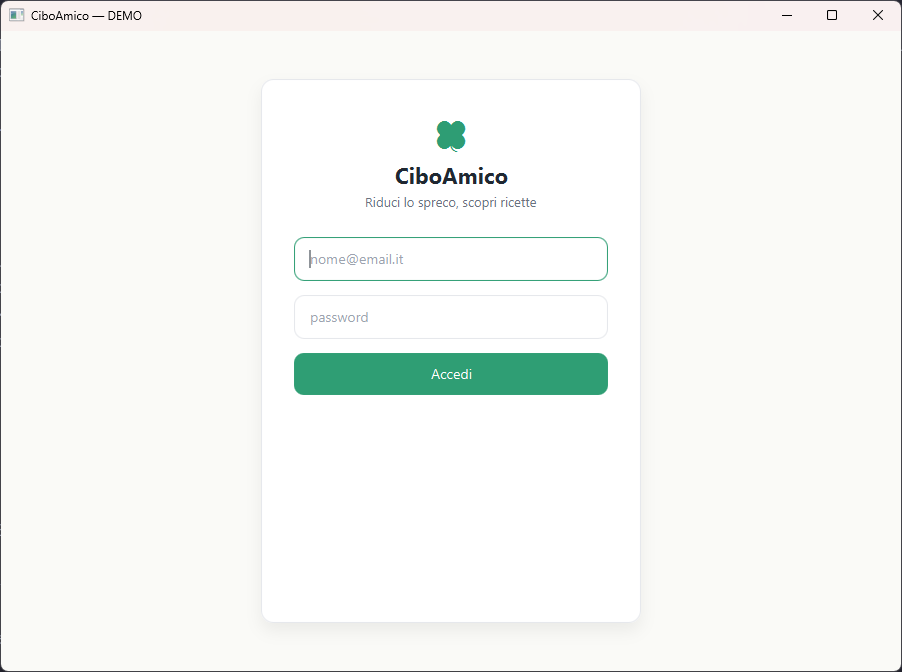
\includegraphics[width=0.8\textwidth]{figures/schermata-login.png}
    \caption{Authentication screen of the system.}
    \label{fig:sb_login}
\end{figure}

\subsection{Home (Customer)}
Once authentication is completed, the Customer reaches the main dashboard (Home). From here they can access the application features: Recipes, Inventory, Shopping List and Marketplace (UC-04 Order a Product).
\begin{figure}[H]
    \centering
    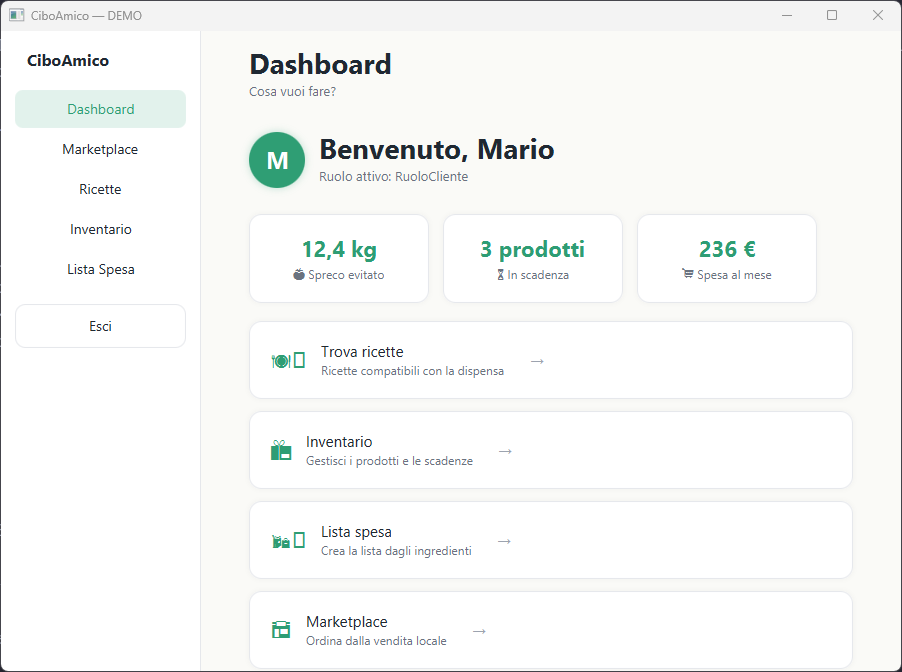
\includegraphics[width=0.8\textwidth]{figures/schermata-home.png}
    \caption{Main dashboard: access to the application features.}
    \label{fig:sb_home}
\end{figure}

\section{Purchases and Marketplace (UC-04 Order a Product)}

\subsection{Marketplace (Product Catalog)}
The area dedicated to direct purchase shows the catalog of local vendor products. The side panel allows the user to select a product to order and, optionally, a promotional voucher.
\begin{figure}[H]
    \centering
    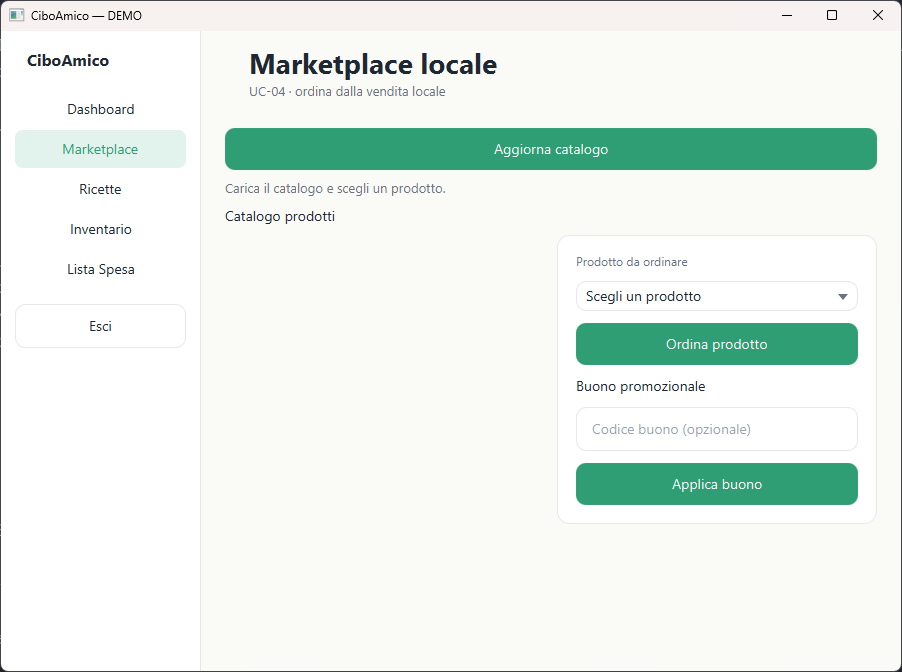
\includegraphics[width=0.8\textwidth]{figures/schermata-marketplace.png}
    \caption{Marketplace: local product catalog and purchase panel.}
    \label{fig:sb_marketplace}
\end{figure}

\subsection{Order a Product}
After selecting a product from the catalog and loading the list (button \emph{Refresh catalog}), the Customer chooses the product in the \emph{Product to order} panel. If they insert a voucher code and press \emph{Apply voucher}, the system validates the voucher and recalculates the total by applying the discount (extension \emph{Order a Product}); by pressing \emph{Order product} the flow proceeds.
\begin{figure}[H]
    \centering
    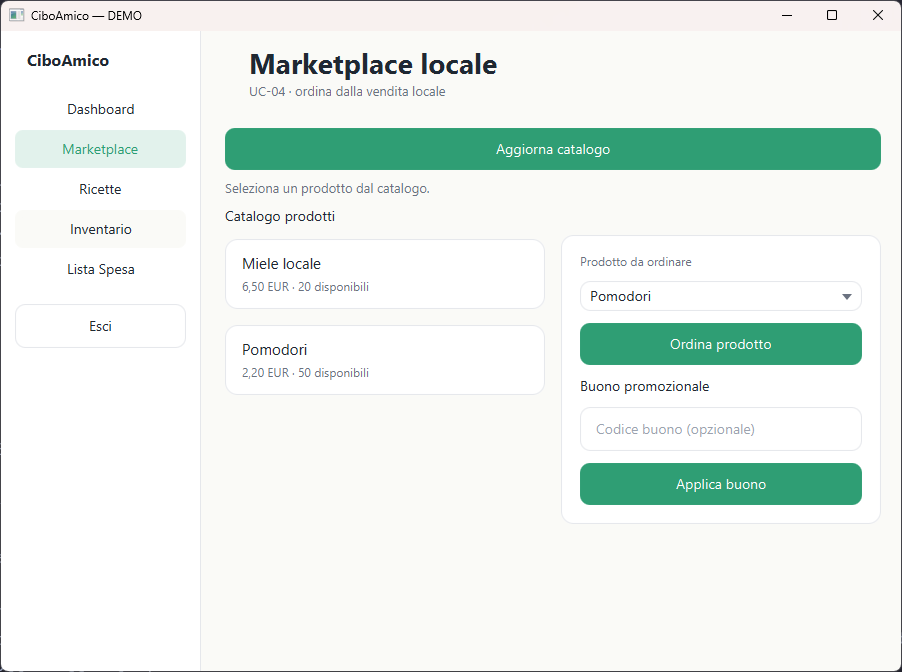
\includegraphics[width=0.8\textwidth]{figures/schermata-ordine.png}
    \caption{Purchase screen with the selected product and the promotional voucher field.}
    \label{fig:sb_ordine}
\end{figure}

\subsection{Payment (step 6)}
Once the order is confirmed, the interface moves to the payment screen: the user inserts the card data (number, holder, expiry date and CVV) and authorizes the debit; the outcome is shown inline in the same view, as required by extension \textbf{6a} (rejected payment) of the use case.
\begin{figure}[H]
    \centering
    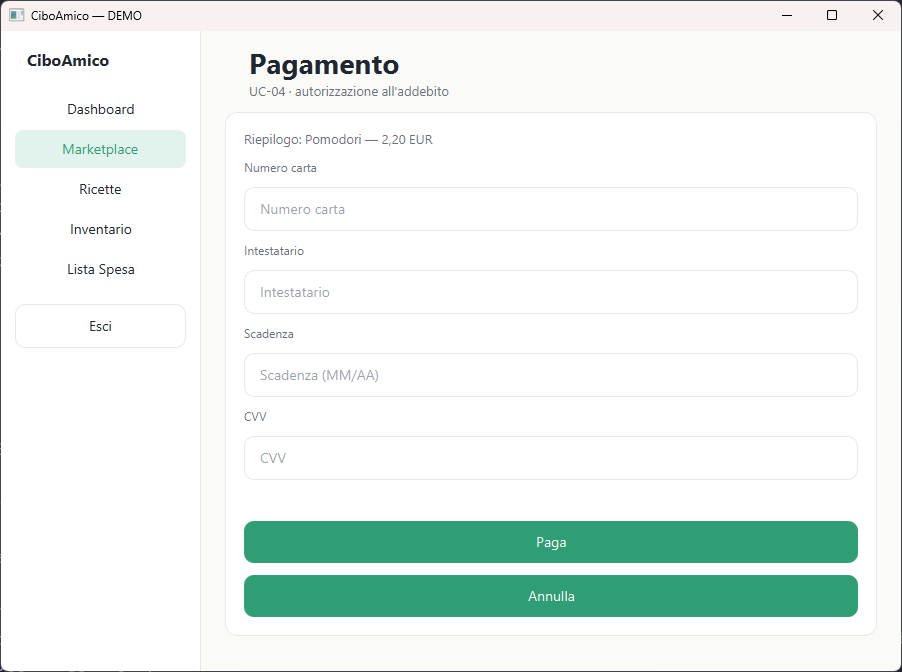
\includegraphics[width=0.8\textwidth]{figures/schermata-payment.png}
    \caption{Payment screen (card data and debit authorization).}
    \label{fig:sb_payment}
\end{figure}
